\chapter{Frontend}
\label{chap_frontend}
In diesem Kapitel wird die prototypische Entwicklung des Frontend beschrieben. Dabei werden anhand der verschiedenen Bereiche die Umsetzung der
Projektstruktur und die Funktionsweise des Programmes erläutert.

\section{Login}
Da die Software, wie in den Projektzielen erwähnt, nicht nur intern im Büro sondern auch von extern aus erreichbar sein muss, ist es nötig, eine Authentifizierung einzurichten damit Unbefugte keine Möglichkeiten haben die Daten zu verändern oder einzusehen. Um die Software nutzen zu können, benötigt der Bearbeiter eine gültige Kombination aus E-Mail Adresse und Passwort. Schon bei der Eingabe der Daten wird überprüft, ob die Felder leer sind oder es sich überhaupt um eine E-Mail Adresse handelt. Dabei wird abgefragt, ob ein \url{@}-Zeichen vorhanden ist und ob darauf ein Punkt folgt.
Sobald das Formular abgeschickt wurde, werden die Daten zunächst im \texttt{login.js} Controller entgegengenommen. Von da aus werden diese an den Authentication-Service weitergegeben wo sie an das Backend weitergereicht werden. In Firebase werden sie dann mit den hinterlegten Daten verglichen. Sind E-Mail Adresse und Passwort nicht korrekt oder nicht vorhanden, wird eine Fehlermeldung zurückgegeben die der Controller im View anzeigt. Sofern alle Angaben korrekt sind, wird der Nutzer weiter zu der Hauptseite geleitet.
Da es sich hierbei um eine betriebsinterne Software handelt, wird eine Registrierung nicht benötigt. Die E-Mail-Adresse und das Passwort werden manuell im Backend hinzugefügt, bearbeitet oder entfernt. Die Folgende Abbildung \ref{frontend_login} zeigt, wie der Anmeldebildschirm aussieht.

\begin{figure}[H]
\centering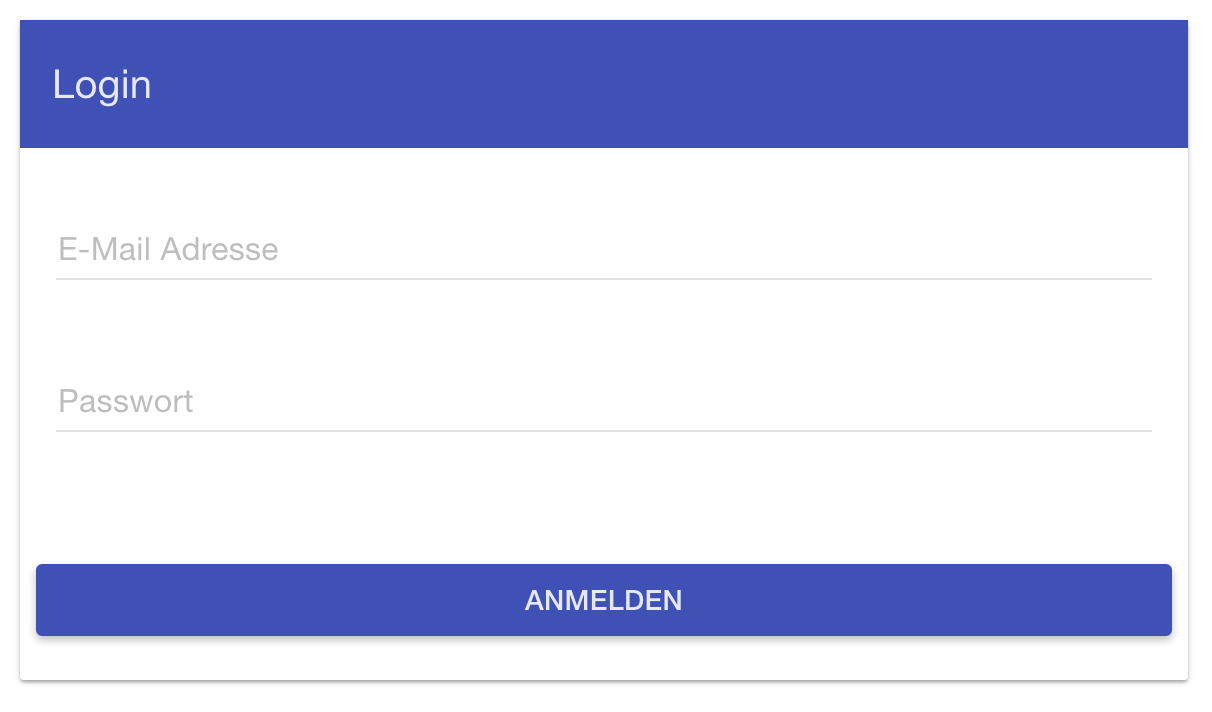
\includegraphics[width=0.5\textwidth]{images/frontend_login.png}
\caption{Anmeldeformular}
\label{frontend_login}
\end{figure}

\section{Hauptseite}
Aus den in den Projektzielen gesteckten Bedingungen ergibt sich die in Abbildung \ref{frontend_mainpage} gezeigte Hauptseite. Diese ist schlicht aufgebaut bietet jedoch gleichzeitig alle gewünschten Funktionen, die mit einem Klick erreicht werden können.

\begin{figure}[H]
\centering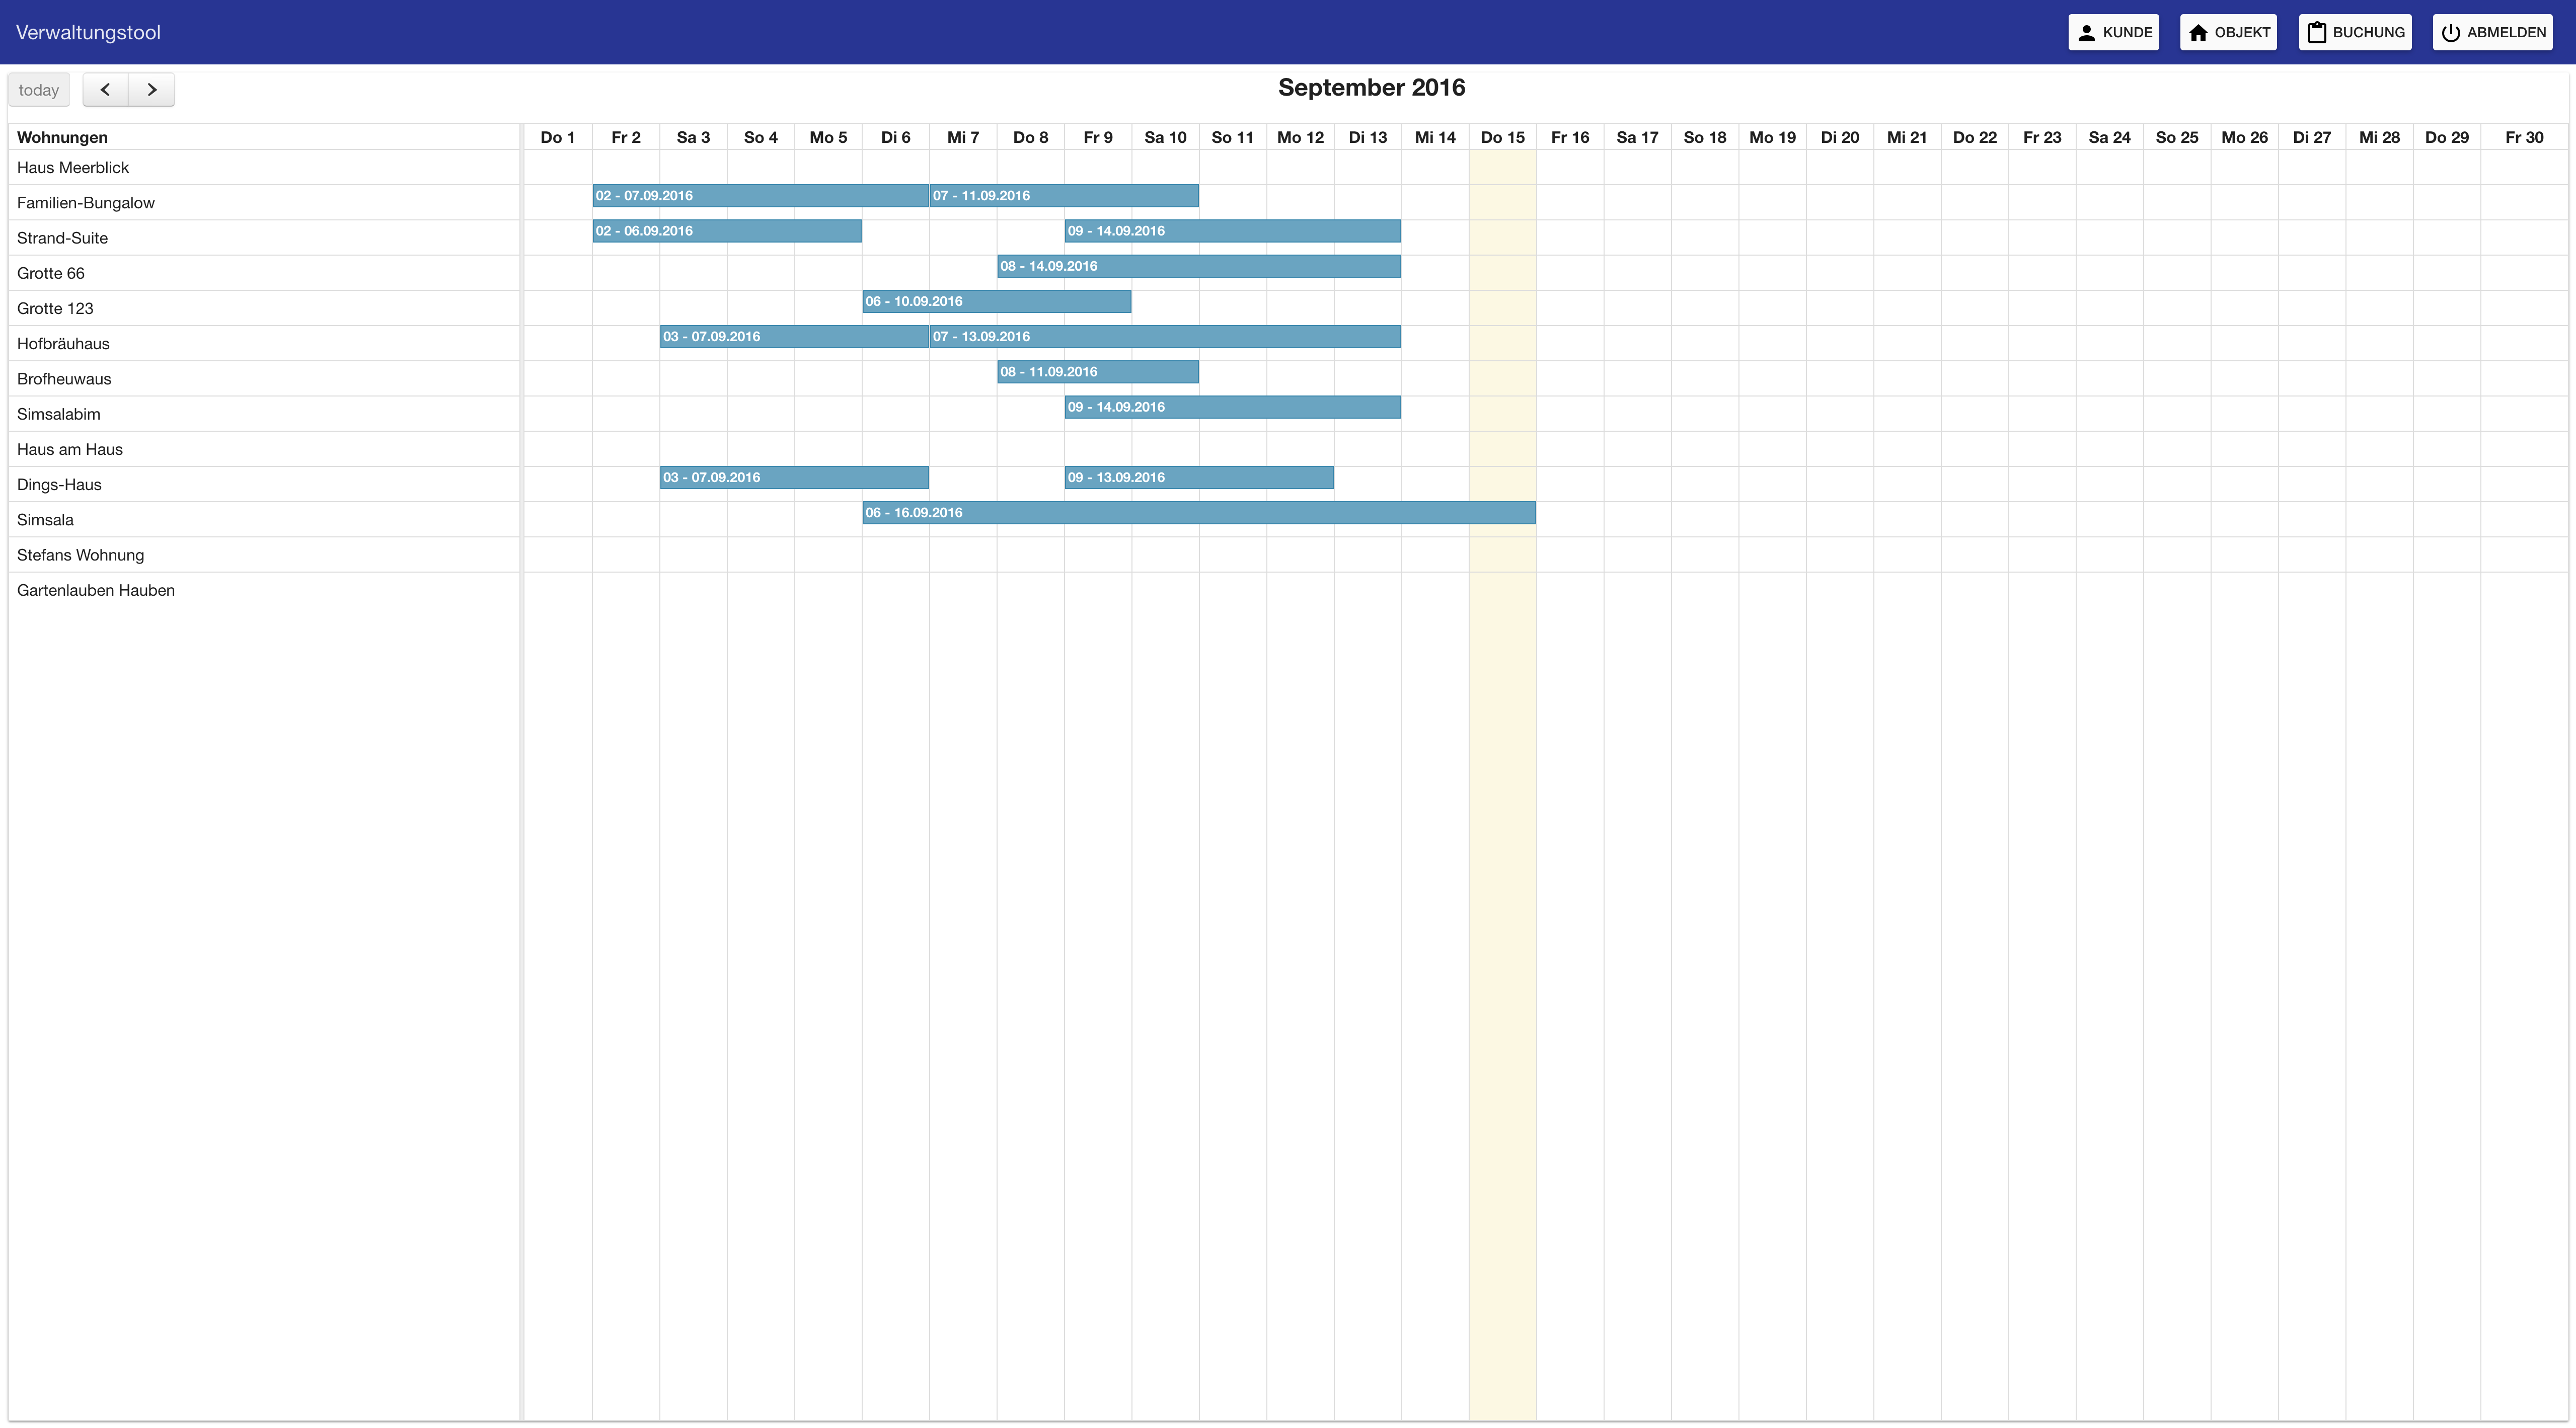
\includegraphics[width=1\textwidth]{images/frontend_mainpage.png}
\caption{Hauptseite}
\label{frontend_mainpage}
\end{figure}

\subsection{Header}
Im Kopfbereich befinden sich neben dem Programm-Name auch folgende vier Button:

\begin{description}
\item[Kunde]\hfill \\
Ein Dialog öffnet sich in dem Kunden hinzugefügt werden können. Nach einer Suche ist das Bearbeitung und Löschen ebenfalls möglich.
\item[Objekt]\hfill \\ 
Ein Dialog öffnet sich in dem eine neue Ferienwohnung / Haus hinzugefügt werden kann. 
\item[Buchung]\hfill \\ 
Ein Dialog öffnet sich in dem eine neue Buchung hinzugefügt werden kann. 
\item[Logout]\hfill \\ 
Nach der Bestätigung eines Dialogs wird der Nutzer abgemeldet und auf die Login-Seite verwiesen. 
\end{description}

Sobald die Fenstergröße kleiner ist oder die Größe eines durchschnittlichen Tablets erreicht wurde, werden die Buttons im Kopfbereich ausgeblendet
(Abbildung \ref{frontend_header_small}). Stattdessen erscheint ein Menüsymbol das bei Klick eine Seitennavigation einblendet in der sich alle Buttons befinden
 (Abbildung \ref{frontend_header_small_navigation}).

\begin{figure}[H]
    \centering
    \begin{minipage}[t]{0.49\linewidth}
        \centering
        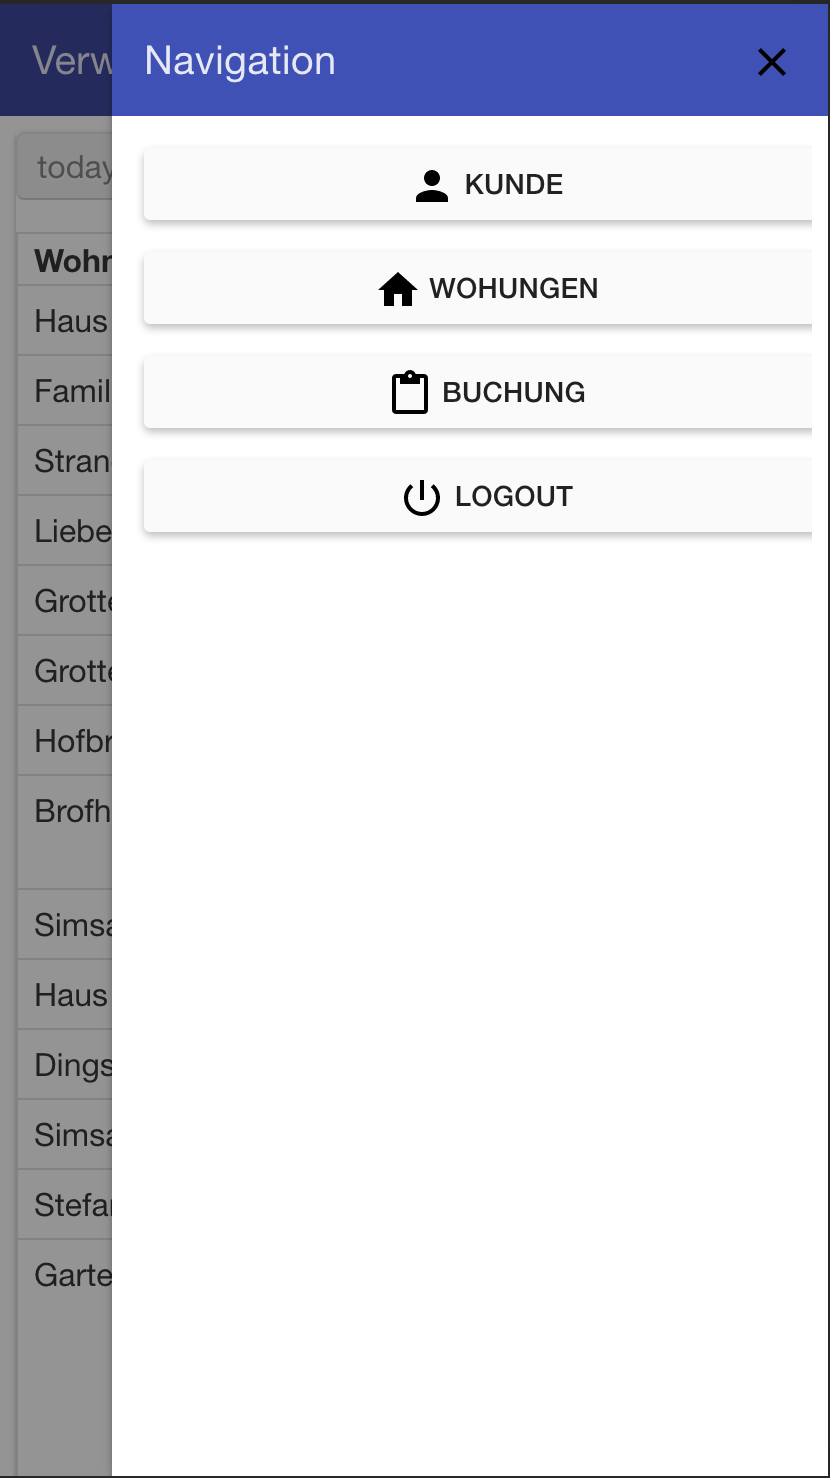
\includegraphics[width=\linewidth]{images/frontend_header_small.png}
        \caption{Ansicht auf Mobilgeräten}
        \label{frontend_header_small}
    \end{minipage}
    \hfill
    \begin{minipage}[t]{0.49\linewidth}
        \centering
        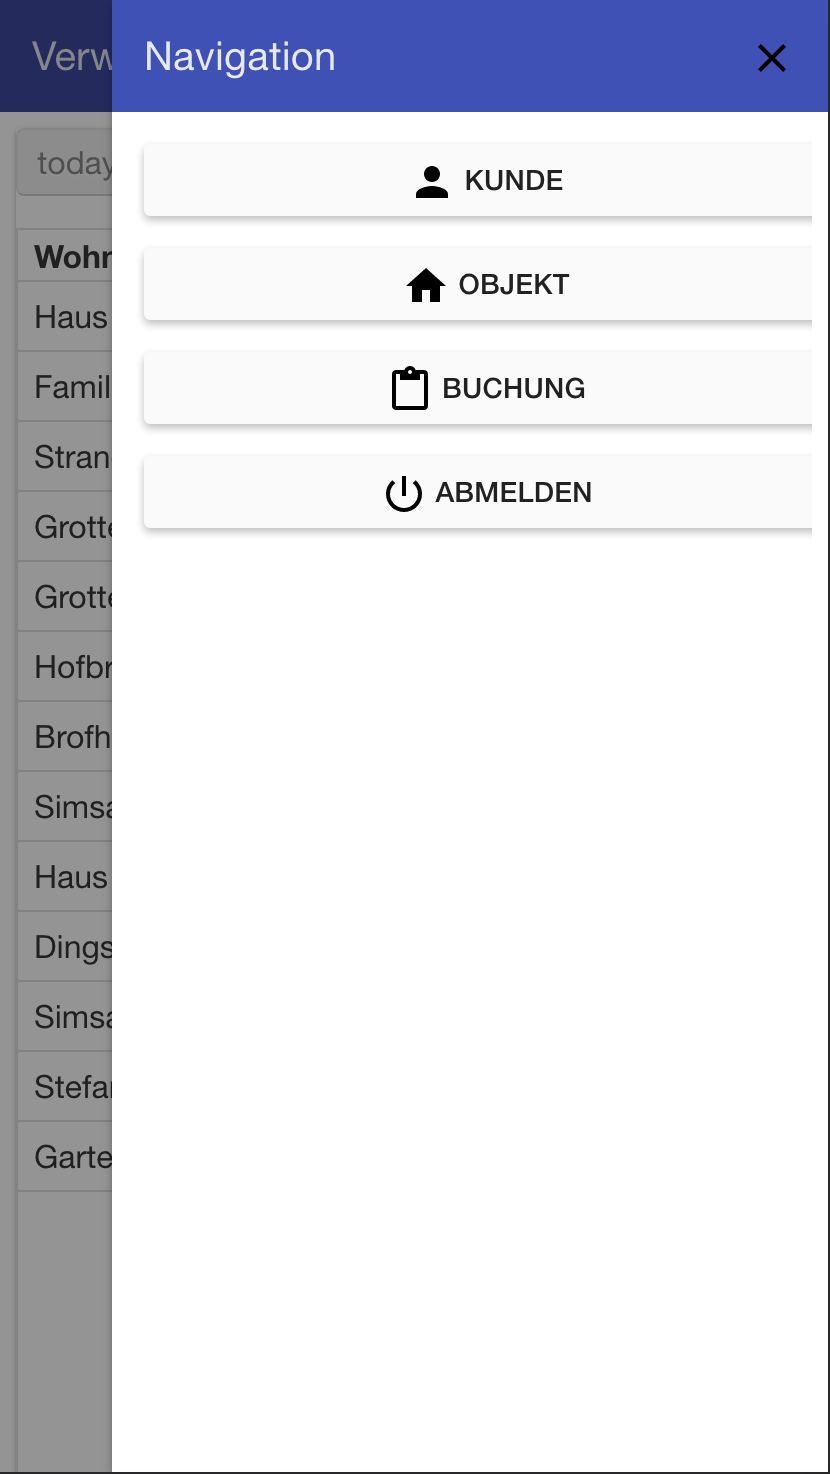
\includegraphics[width=\linewidth]{images/frontend_header_small_navigation.png}
        \caption{Seitennavigation auf Mobilgeräten}
        \label{frontend_header_small_navigation}
    \end{minipage}
\end{figure}


\subsection{Main}
In der Main-View befindet sich der eigentliche Kalender, in dem in einer Monatsübersicht die Buchungen dargestellt werden.
Dieser teilt sich in folgende zwei Bereiche:
\begin{description}
\item[Objektübersicht]\hfill \\
Alle Buchungsobjekte werden auf der linken Seite in Form einer Liste dargestellt.
\item[Buchungsübersicht]\hfill \\ 
Alle Tage des aktuellen Monats werden als Spalten dargestellt. Die Buchungen werden als Blöcke angezeigt und verbinden die einzelnen Tage an denen das Objekt gebucht ist.  
\end{description}

\section{Kunde}
Zusammen mit dem Objekt bildet der Kunde eine Buchung. Für die Kundeninformationen wurden alle Felder aus dem Projektzielen implementiert (Abbildung \ref{frontend_customer_new}). Zudem sind alle Felder ausgenommen der Zusatzinformationen und der Firma pflicht. Diese werden beim Abschicken des Formulars geprüft, ob sie leer sind. Um die Eingabe des Geburtstages zu vereinfachen wurde jeweils für Tag, Monat und Jahr ein Dropdown-Menü bereitgestellt. Da das Mindestalter für Buchungen 18 Jahre ist, ist das höchste auszuwählende Jahr immer 18 Jahre vom aktuellen aus gerechnet. Alle Zeitangaben werden im UNIX TIMESTAMP gespeichert. Sind alle Felder korrekt ausgefüllt, kann das Formular abgeschickt werden. Sobald die \texttt{submit} Funktion im Controller aufgerufen wird, werden alle Felder aus dem View in einem \texttt{customer} JSON-Objekt gespeichert. Diese werden dem \texttt{Customer} Model übergeben und das Dialogfenster geschlossen.

\begin{lstlisting}[language=JavaScript, label=code_exampleRegistrationRequest, caption=submit Methode im customer Controller]
		$scope.submit = function () {
            $scope.birthday = new Date($scope.yearOfBirth + '-' + $scope.monthOfBirth + '-' + $scope.dayOfBirth).getTime();
            var customer = new Customer({
                Company: $scope.company,
                FirstName: $scope.firstname,
                LastName: $scope.lastname,
                BirthDate: $scope.birthday,
                Street: $scope.street,
                City: $scope.city,
                ZipCode: $scope.zipcode,
                Email: $scope.email,
                Phone: $scope.phone,
                Custom: $scope.custom,
                Id: $scope.customerID || undefined
            });
            Customers.upsert(customer);
            $scope.hide();
            $rootScope.$broadcast('showToast');
        };
\end{lstlisting}

Soll ein bestehender Kunde bearbeitet werden, wie in Abbildung \ref{frontend_customer_edit} zu sehen, muss dieser zunächst über das in Abbildung \ref{frontend_customer_search}
gezeigte Suchfeld ermittelt werden. Mit einem Klick auf das Lupensymbol im Kopfbereich des Dialog wird die Suchleiste jeweils ein- oder ausgeblendet. Sobald das Suchfeld
fokussiert wird, wird eine Funktion im Controller angestoßen, welche alle Kunden mit Vor und Nachname als Auswahlmöglichkeit auflistet. Dafür wird im Model die Liste aller
Kunden aus der Datenbank angefordert. Das Model Liefert dem Controller ein Array mit allen Kunden als JSON-Objekt. Bei einer hohen Anzahl an Kunden kann sich die Suche durchaus schwierig
gestalten. Aus diesem Grund kann der Kunde durch eintippen von Buchstaben gefiltert werden. Jeder weitere Buchstabe schränkt die Suche nach dem Kunden ein und es
werden nur Kunden angezeigt dessen Nachname die eingegebene Zeichenkette beinhalten.

\begin{figure}[H]
\centering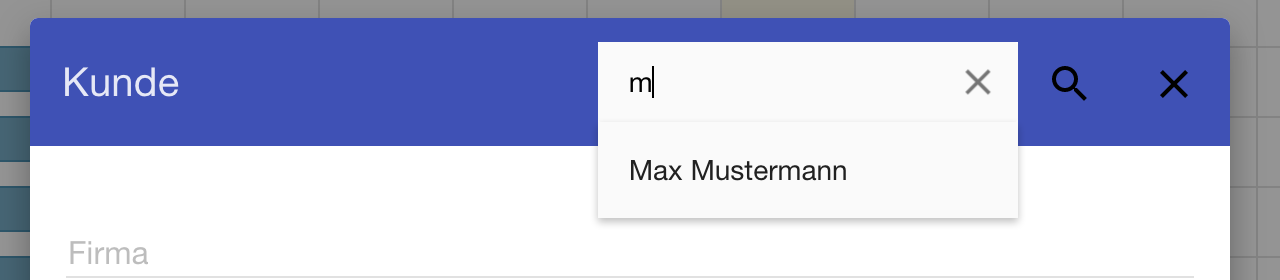
\includegraphics[width=0.5\textwidth]{images/frontend_customer_search.png}
\caption{Kundensuche}
\label{frontend_customer_search}
\end{figure}

\begin{figure}[H]
    \centering
    \begin{minipage}[t]{0.49\linewidth}
        \centering
        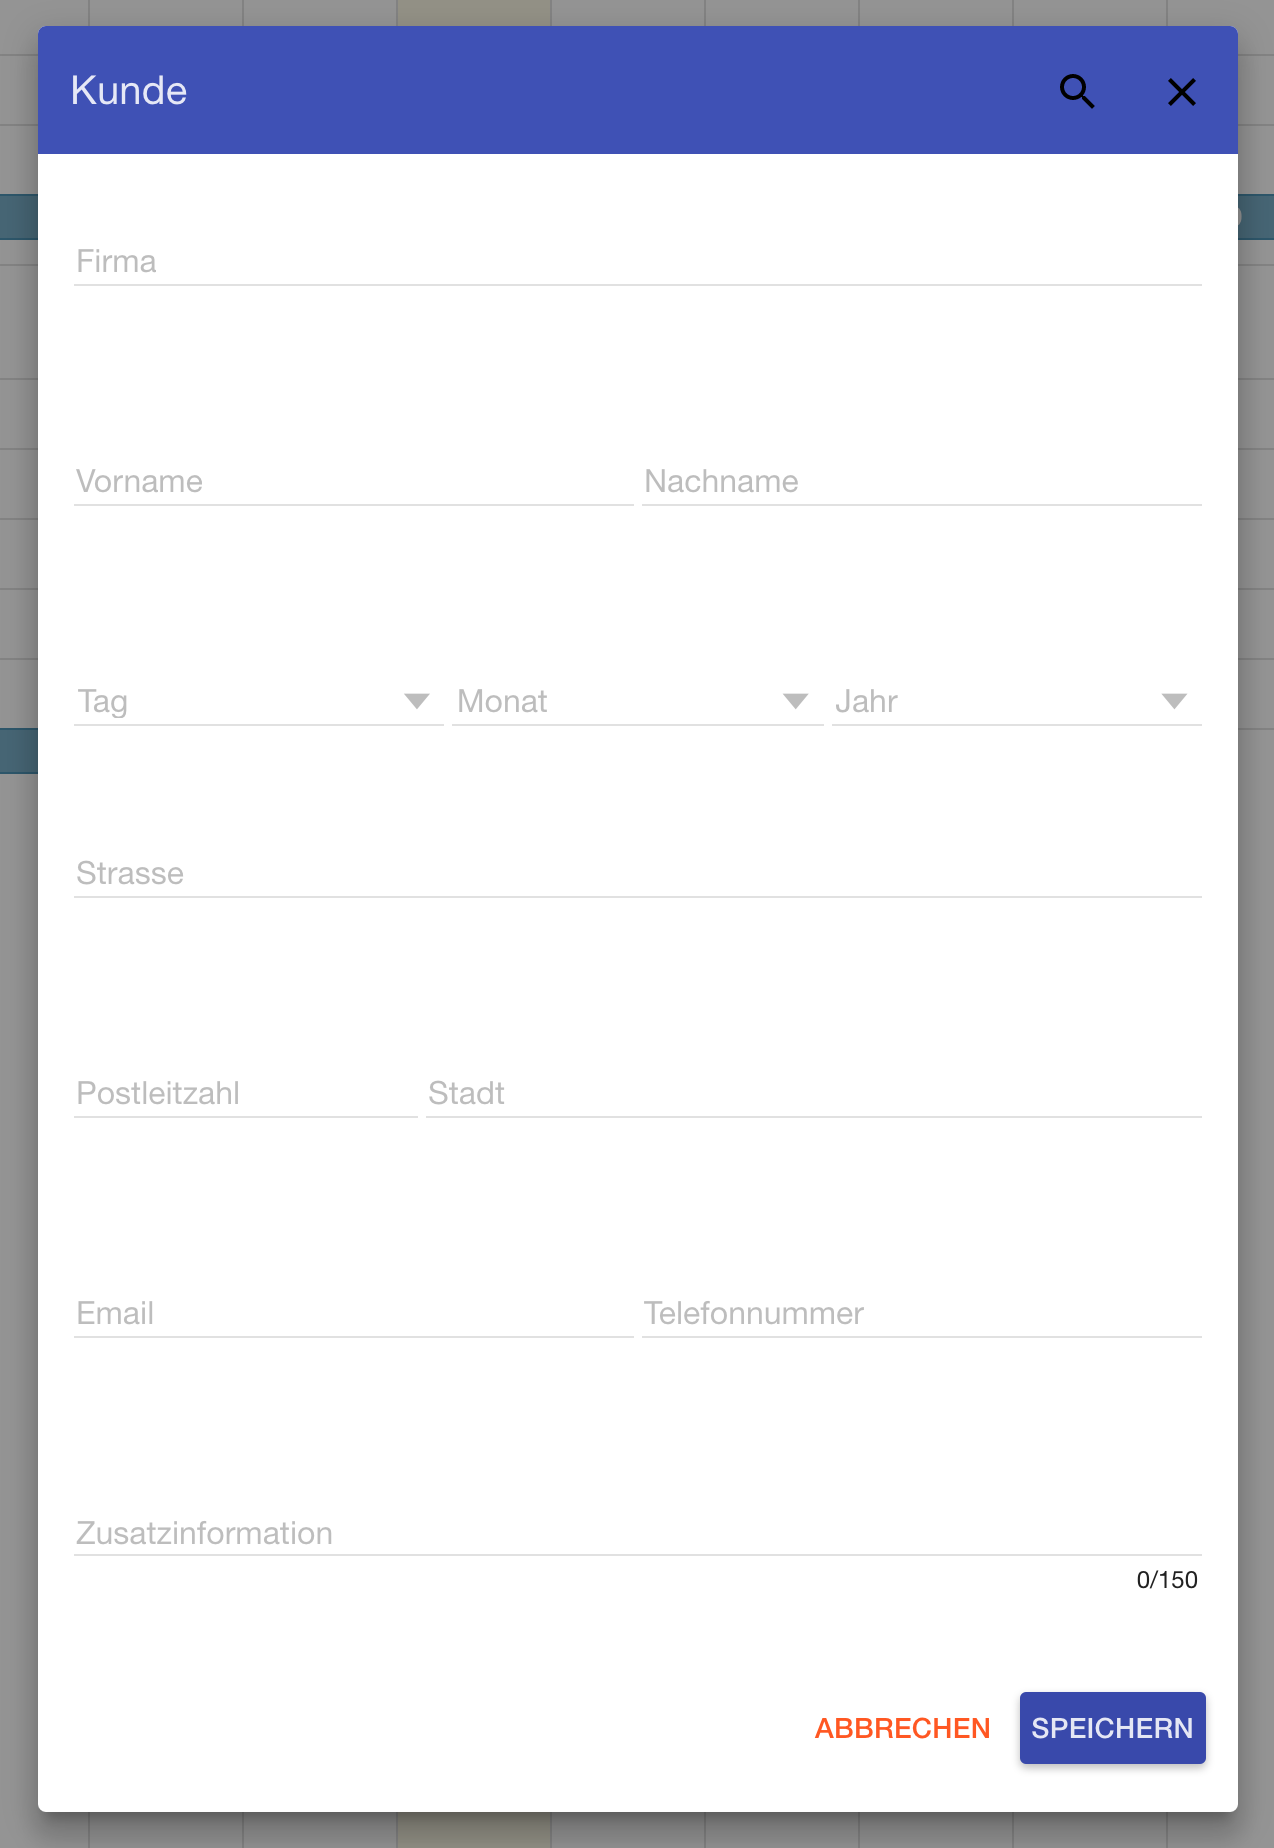
\includegraphics[width=\linewidth]{images/frontend_customer_new.png}
        \caption{Neuen Kunden erstellen}
        \label{frontend_customer_new}
    \end{minipage}
    \hfill
    \begin{minipage}[t]{0.49\linewidth}
        \centering
        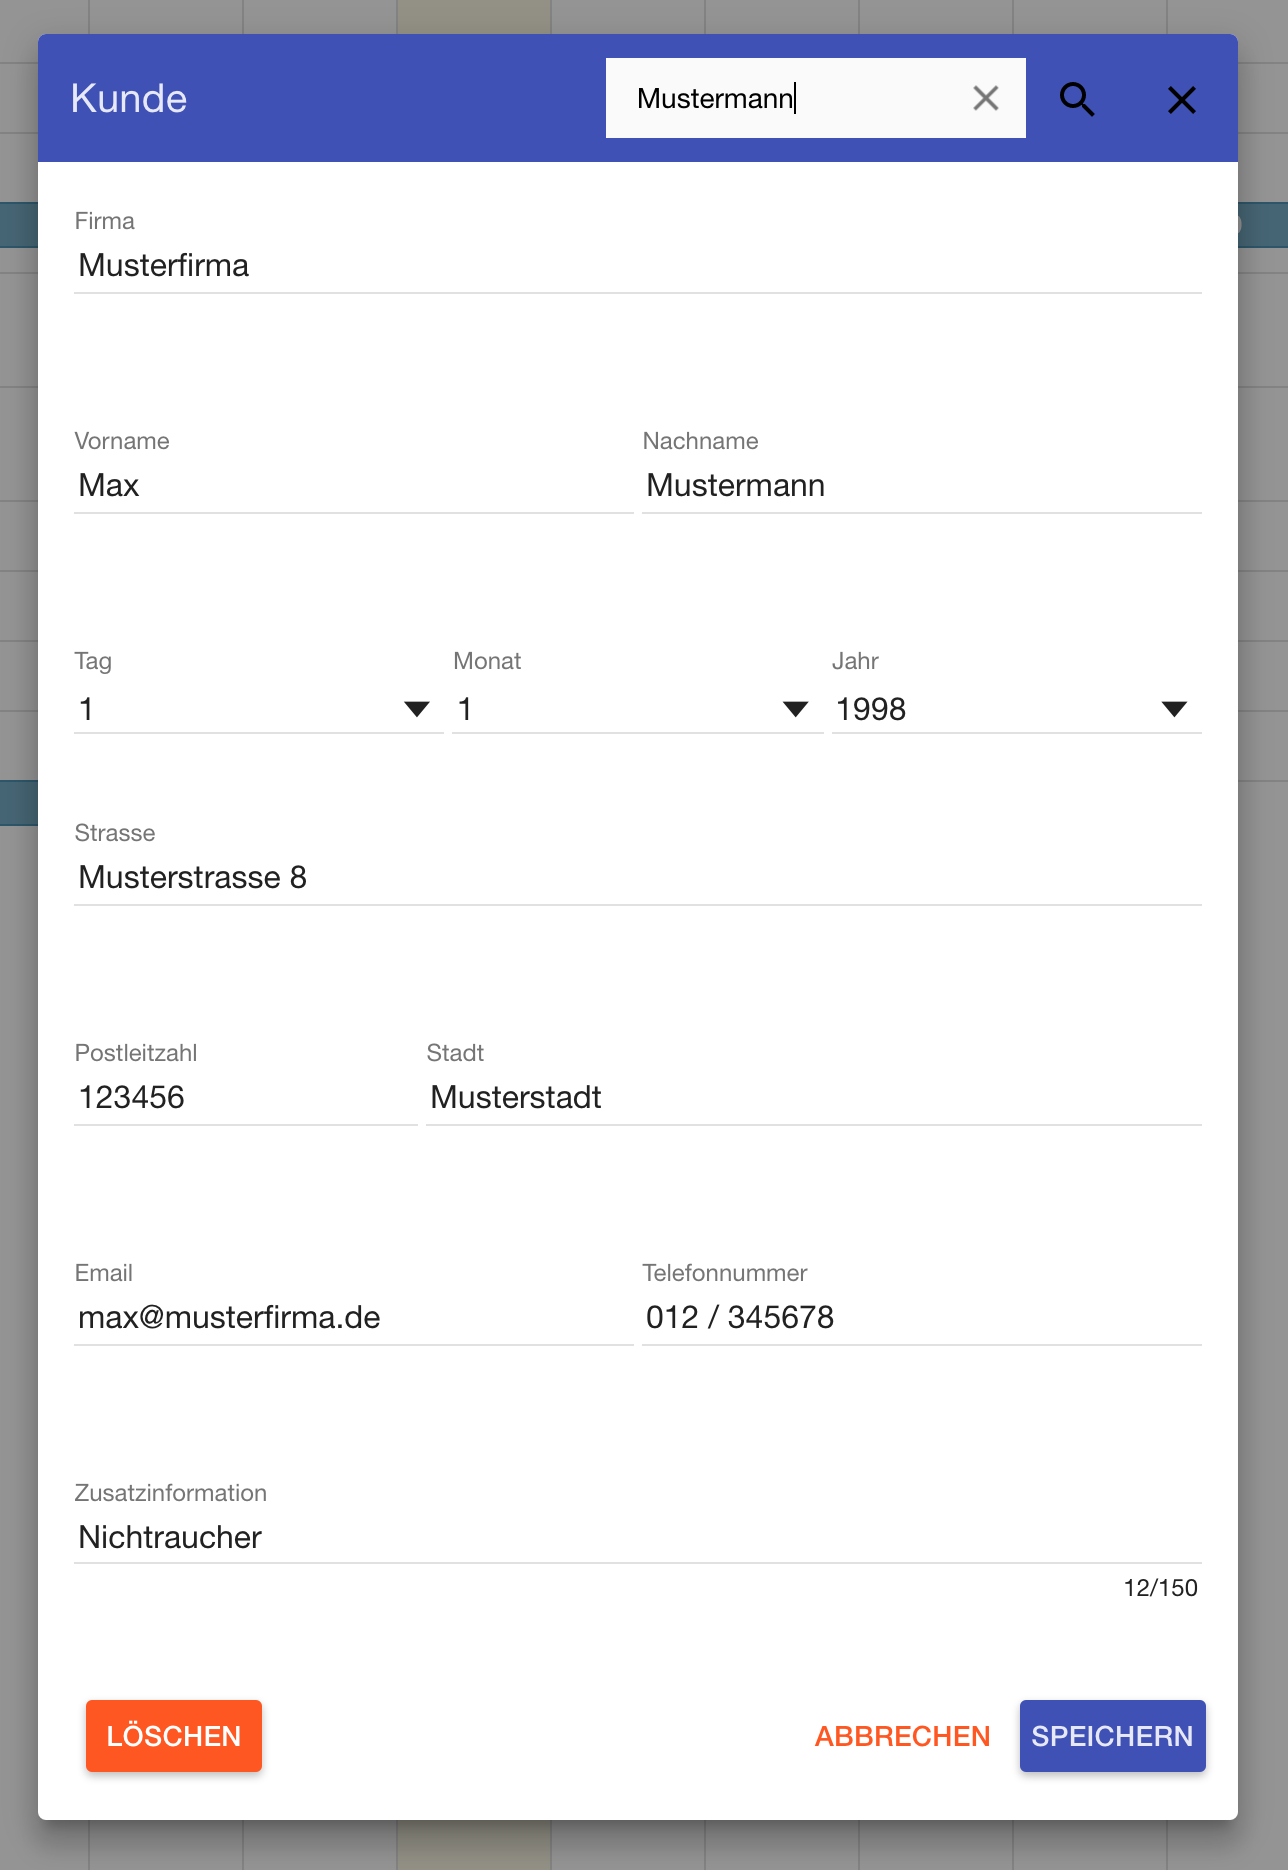
\includegraphics[width=\linewidth]{images/frontend_customer_edit.png}
        \caption{Kunden bearbeiten}
        \label{frontend_customer_edit}
    \end{minipage}
\end{figure}

Wurde ein Kunde ausgewählt, werden alle Daten aus dem JSON-Objekt ausgelesen und in die jeweiligen Input Felder eingefügt. Gleichzeitig wird ein Button zum löschen des Kunden angezeigt. Um ein Fehler beim Löschen vorzubeugen muss zusätzlich noch ein Dialog bestätigt werden. Ist das der Fall, übergibt der Controller dem Model die UUID des Kunden in einer \texttt{delete} Funktion. 

Wenn Daten verändert wurden können diese wie auch beim Hinzufügen eines neuen Kunden ganz normal bestätigt werden. Im Controller wird die \texttt{upsert} Methode des Model aufgerufen. Je nachdem, ob es sich dabei um einen bestehenden Eintrag in der Datenbank handelt oder einen neuen Kunden, wird ein \texttt{Update} oder \texttt{Insert} durchgeführt.

Soll weder ein neuer Kunde hinzugefügt noch ein bestehender bearbeitet werden kann das Dialog über den \grqq Abbrechen\glqq{}  Button, das \grqq X\glqq{}  oder einen
Klick ausserhalb des Dialogs geschlossen werden. Der Controller ruft die \texttt{hide} Methode des Dialogs auf und das Dialogfenster wird ausgeblendet. Dabei werden auch alle Daten aus den Feldern entfernt.

\section{Objekt}
Als Objekt wird eine Ferienwohnung oder Haus bezeichnet. Wie auch beim Kunden können bei einem Objekt verschiedene Informationen gespeichert werden. Die beiden Felder aus den Projektzielen wurden implementiert (Abbildung \ref{frontend_resource_new}). Dazu gehört die Eingabe des Namens und die Personenanzahl in ein Textfeld. Wird das Feld fokussiert, und ohne Eingabe verlassen, erscheint eine Fehlermeldung mit dem Hinweis, dass das Feld auszufüllen ist (Abbildung \ref{frontend_resource_fail}). Wird dieser Hinweis ignoriert und der Nutzer versucht dennoch das Formular abzuschicken überprüft der View, ob alle als Pflicht gekennzeichneten Felder ausgefüllt wurden und der \texttt{submit} Button gedrückt wurde. Ist eines dieser beiden \texttt{false}, wird das Formular nicht abgeschickt.

\begin{figure}[H]
    \centering
    \begin{minipage}[t]{0.49\linewidth}
        \centering
        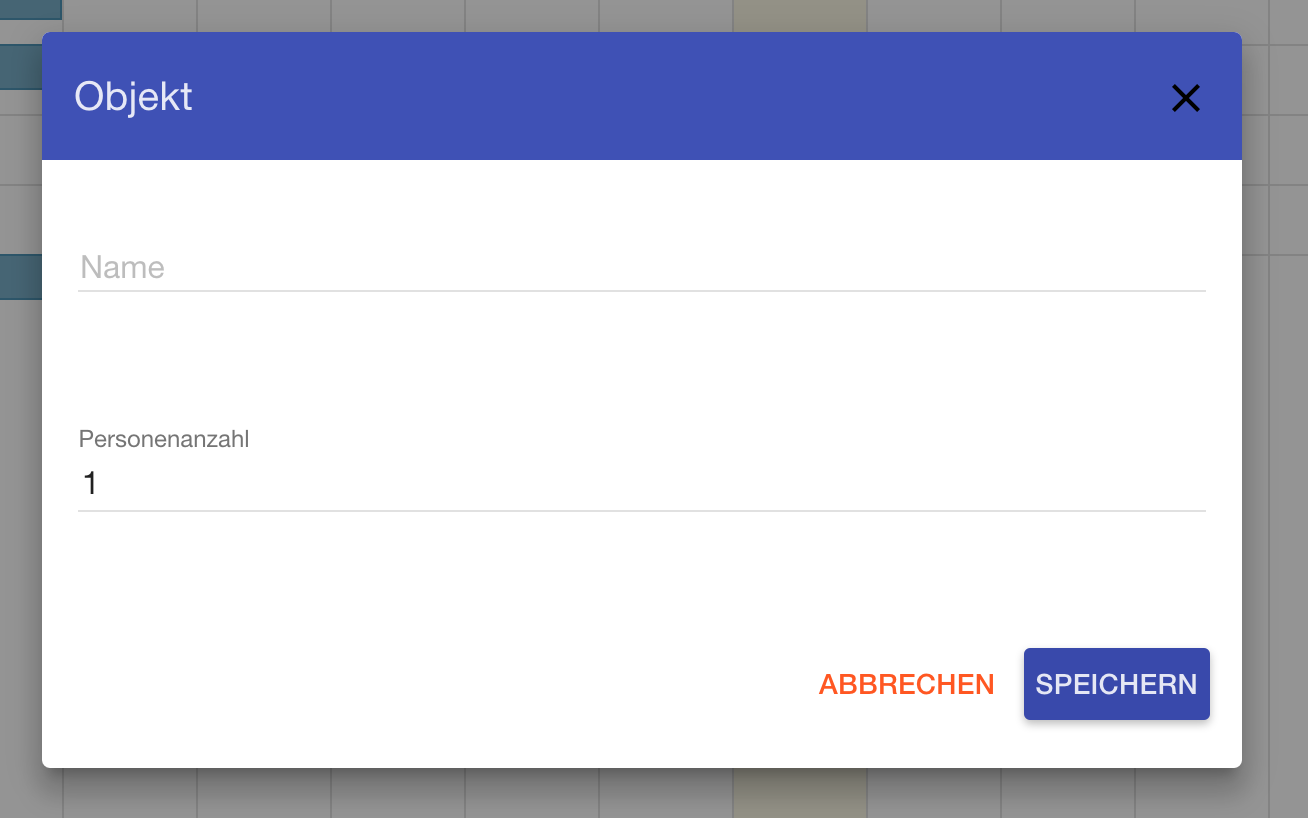
\includegraphics[width=\linewidth]{images/frontend_resource_new.png}
        \caption{Objekt erstellen}
        \label{frontend_resource_new}
    \end{minipage}
    \hfill
    \begin{minipage}[t]{0.49\linewidth}
        \centering
        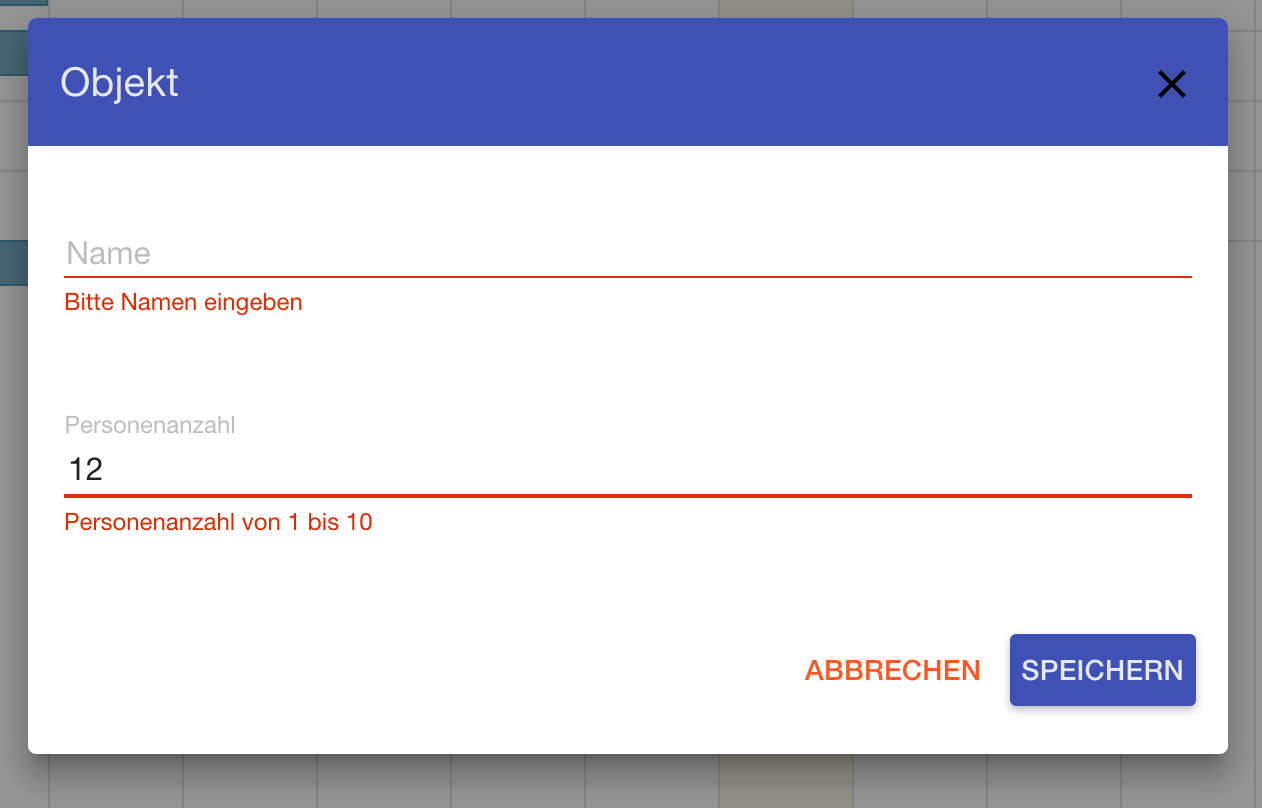
\includegraphics[width=\linewidth]{images/frontend_resource_fail.png}
        \caption{Objekt bearbeiten}
		\label{frontend_resource_fail}
    \end{minipage}
\end{figure}

 Auch bei der Angabe der maximalen Personenanzahl wurde darauf geachtet fehlerhafte Eingaben abzufangen. Standardmäßig ist eine Mindestpersonenanzahl von 1 eingestellt. Der Nutzer hat die Möglichkeit mit Hilfe von Pfeilen den Wert zu Verändern. Die Maximale Anzahl von Personen ist 10 pro Objekt. Da es auch möglich ist Manuell eine Zahl einzugeben wird ebenfalls überprüft, ob sich die Zahl zwischen 1 und 10 befindet. Ist dies nicht der Fall wird ein Hinweis ausgegeben und das Formular kann nicht abgeschickt werden. 
 Sind alle Angaben korrekt und der \texttt{submit} Button wird betätigt, wird das Formular abgeschickt. Im Controller wird eine Methode aufgerufen in der die Daten aus den Feldern in ein JSON-Objekt gespeichert werden. Dieses wird der \texttt{upsert} Methode des Models übergeben. Die Überprüfung der Personenanzahl findet im View statt.
 
 \begin{lstlisting}[language=HTML, label=code_exampleRegistrationRequest, caption=Validierung der Personenanzahl im View]
		<input required type="number" step="any" name="rate" ng-model="size" min="1" max="10"  />
            <div ng-messages="resourceForm.size.$error">
                <div ng-message="required">Personenanzahl von 1 bis 10</div>
            </div>
\end{lstlisting}
 
Um ein bereits existierendes Objekt bearbeiten zu können muss dies anders als bei den Kunden in der Auflistung im Kalender ausgewählt werden (Abbildung \ref{frontend_resource_edit}). Auch hier werden die Daten anhand der UUID aus der Datenbank geladen und in die Felder eingefügt. Zusätzlich wird der Button zum Löschen des Objektes angezeigt. Die Besonderheit bei der Änderung von Daten ist eine Eigenschaft im JSON-Objekt in dem die Informationen der Felder gespeichert werden. Neben dem Namen und der Personenanzahl wird auch die ID des Objektes gespeichert. Ist, wie bei einer Änderung, bereits eine UUID vorhanden, wird diese als Wert gespeichert. Wird ein Objekt neu hinzugefügt, ist die ID \texttt{undefined}. Diese Information wird in der
\texttt{upsert} Methode des Models abgefragt und dementsprechend ein neues Objekt hinzugefügt oder ein bestehendes aktualisiert.

\begin{figure}[H]
\centering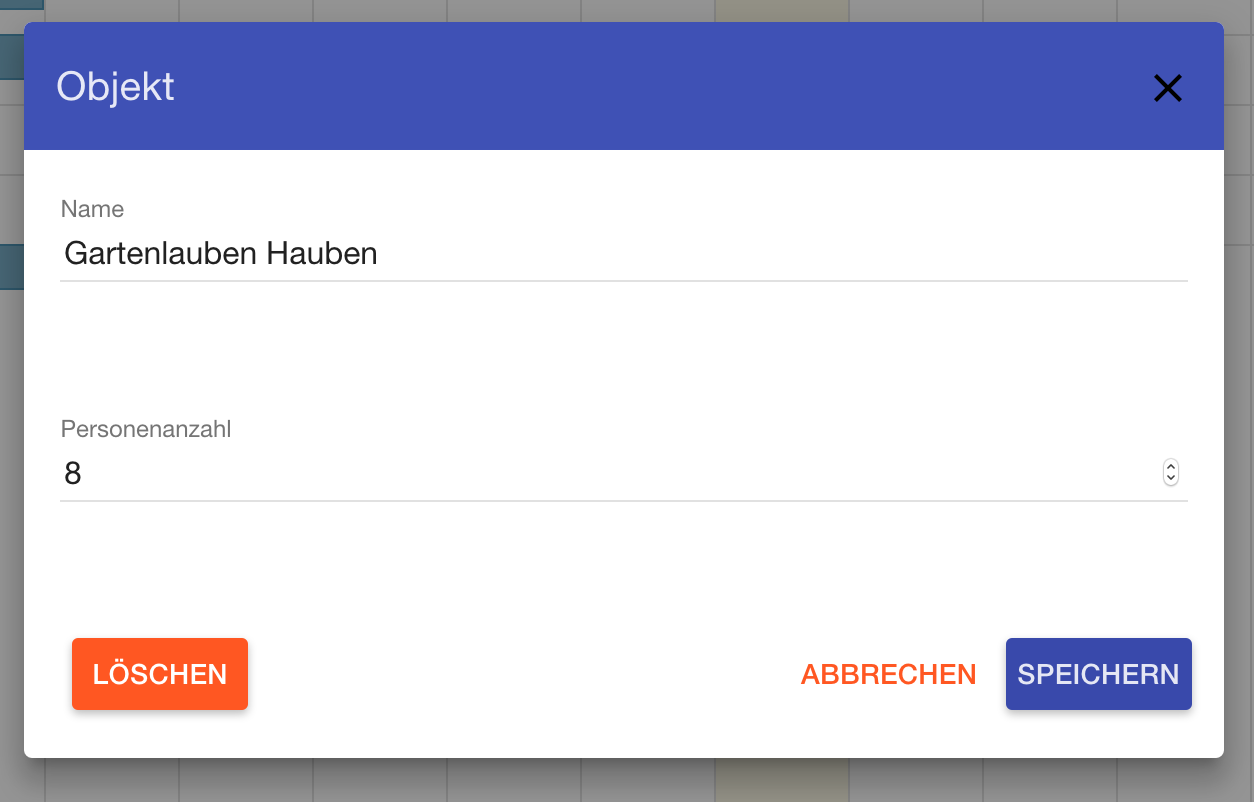
\includegraphics[width=0.5\textwidth]{images/frontend_resource_edit.png}
\caption{Eingabefehler bei Objekt}
\label{frontend_resource_edit}
\end{figure}
  
\section{Buchung}
Eine Buchung ist ein Zusammenschluss aus Kunde, Objekt, Personenanzahl, Startdatum und Enddatum. Wie bei der Bearbeitung von Kunden kann der Nutzer den Kunden und das Objekt über ein Suchfeld filtern und Auswählen. Wenn eine neue Buchung hinzugefügt wird, wird vorerst die Auswahl der Personenanzahl ausgeblendet (Abbildung \ref{frontend_booking_new}). Erst wenn ein Objekt im Suchfeld ausgewählt wurde, wird die Auswahl in form eines Dropdown-Menüs im View angezeigt. Im Controller wird die maximale Personenanzahl des ausgewählten Objektes aus dem JSON-Objekt entnommen und somit die zur Auswahl stehenden Zahlen ermittelt. So zeigt das Dropdown-Menü nur genau die Anzahl von Personen an, die dieses Objekt zur Verfügung stellt.
Für das Startdatum und Enddatum wurden, anders als beim Kunden, ein Datepicker bereit gestellt, der es dem Nutzer erlaubt das Datum durch einfache Auswahl in einem Kalender festzulegen (Abbildung \ref{frontend_booking_calender}). Für diesen ist Standardmäßig das aktuelle Datum eingestellt.

\begin{figure}[H]
    \centering
    \begin{minipage}[t]{0.49\linewidth}
        \centering
        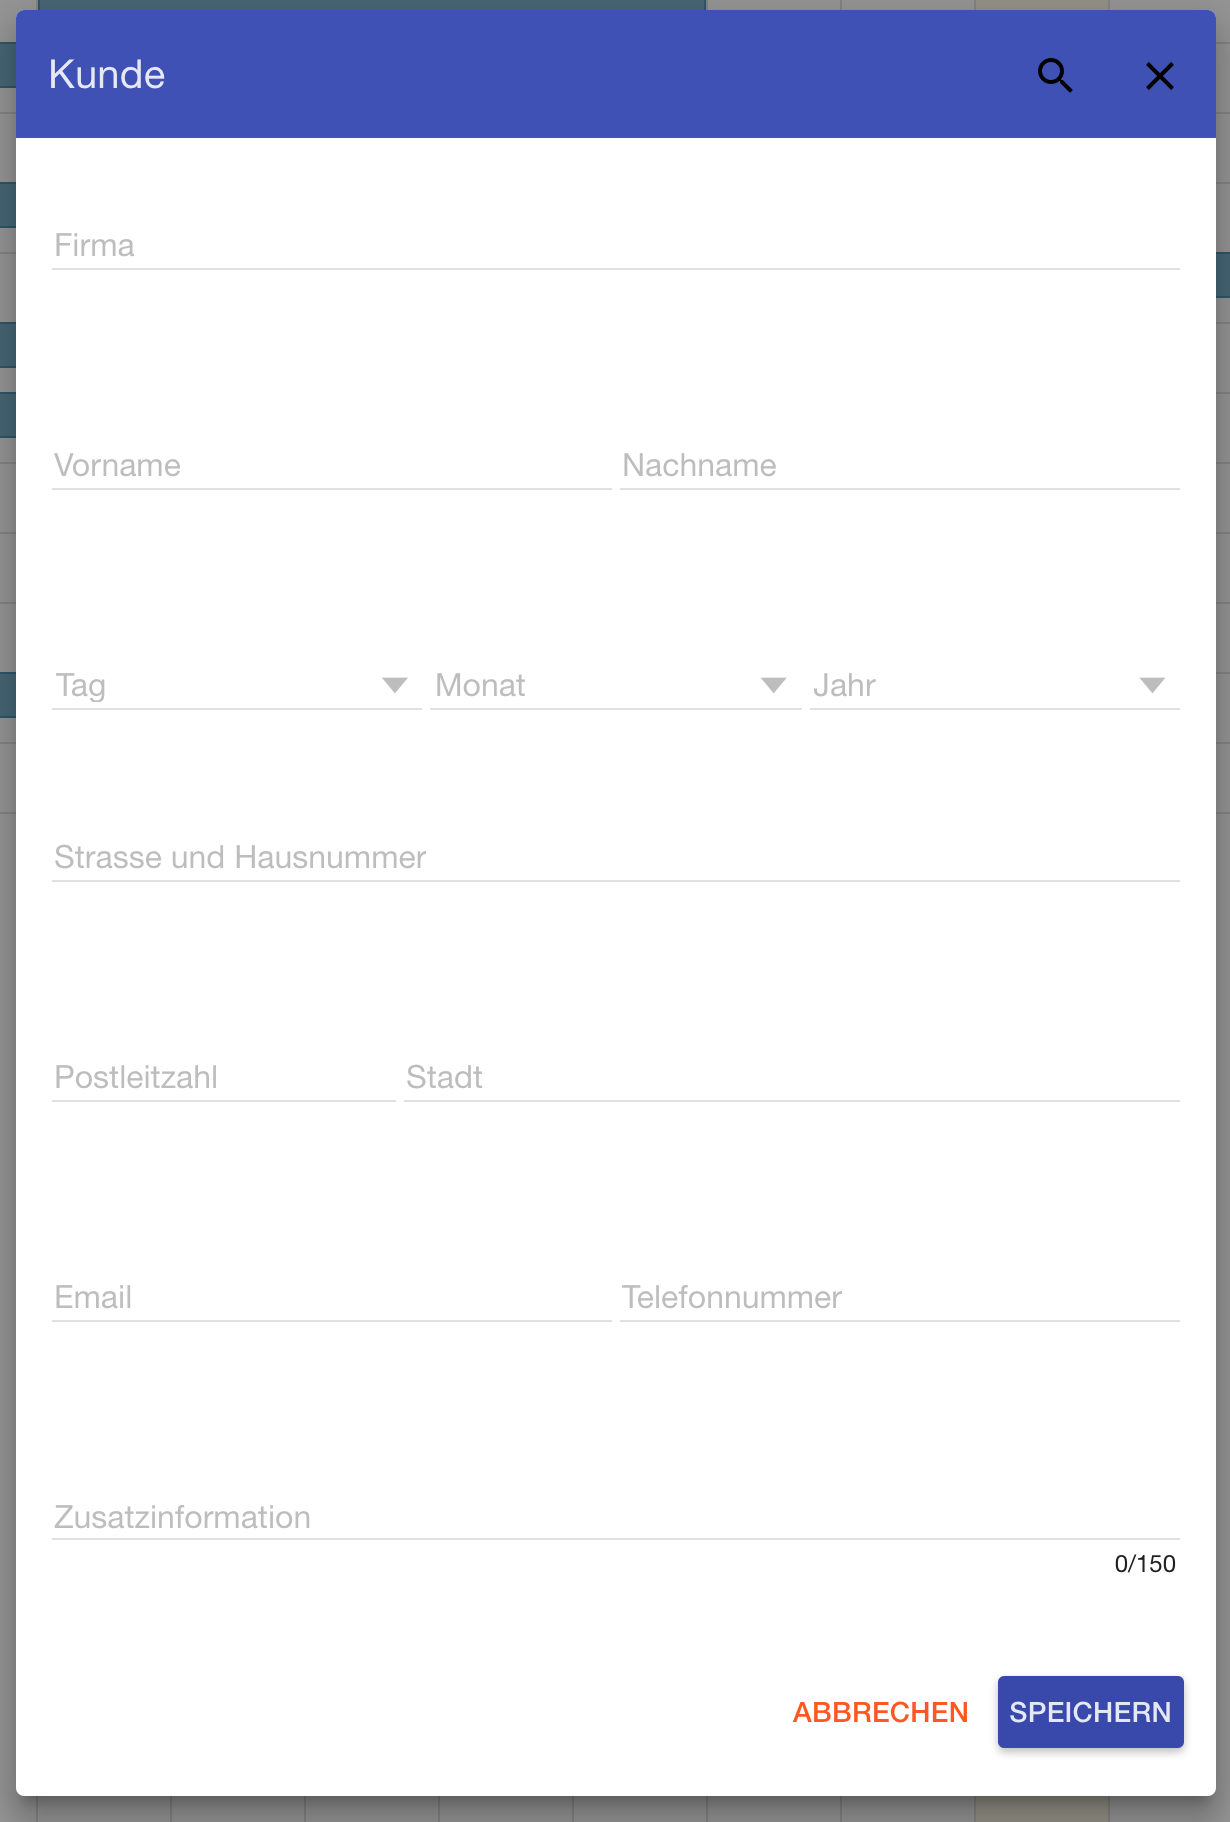
\includegraphics[width=\linewidth]{images/frontend_booking_new.png}
        \caption{Objekt erstellen}
        \label{frontend_booking_new}
    \end{minipage}
    \hfill
    \begin{minipage}[t]{0.49\linewidth}
        \centering
        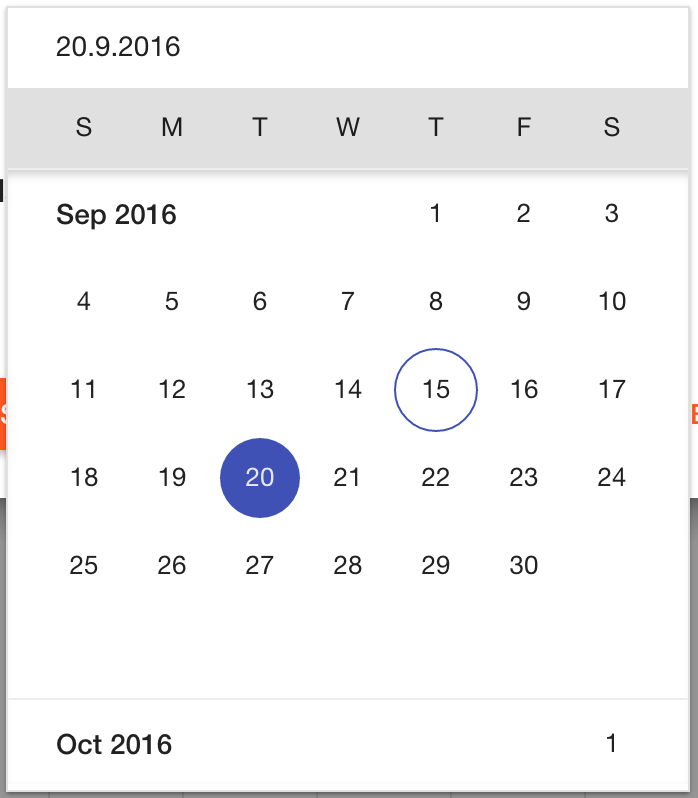
\includegraphics[width=\linewidth]{images/frontend_booking_calender.png}
        \caption{Auswahl des Datum}        
        \label{frontend_booking_calender}
    \end{minipage}
\end{figure}

Um eine Buchung bearbeiten zu können muss diese, anders als beim Kunden oder Objekt, zunächst in der Buchungsübersicht ausgewählt werden. Hier wird die Personenauswahl von beginn an angezeigt und ist mit dem eingetragenem Wert vordefiniert. Auch hier besteht die Möglichkeit, durch bestätigen des Löschen-Dialogs die Buchung aus der Datenbank zu entfernen (Abbildung \ref{frontend_booking_delete_dialog}).

\begin{figure}[H]
    \centering
    \begin{minipage}[t]{0.49\linewidth}
        \centering
        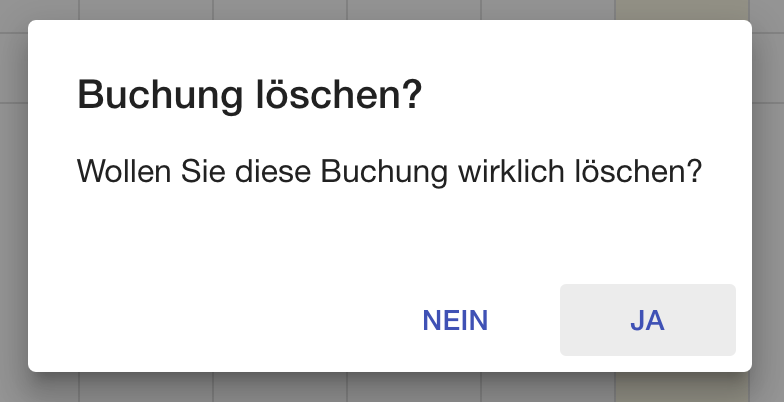
\includegraphics[width=\linewidth]{images/frontend_booking_delete_dialog.png}
        \caption{Objekt erstellen}
        \label{frontend_booking_delete_dialog}
    \end{minipage}
    \hfill
    \begin{minipage}[t]{0.49\linewidth}
        \centering
        
\includegraphics[width=\linewidth]{images/frontend_toast.png}
        \caption{Objekt Fehlereingabe}
         \label{frontend_toast}
    \end{minipage}
\end{figure}

Wird ein Dialog bestätigt, erscheint für drei Sekunden am oberen rechten Fensterrand eine Nachricht (Abbildung \ref{frontend_toast}). Ein sogenannter Toast fährt herunter und zeigt die Erfolgsmeldung und einen Button zum schließen an. In der mobilen Ansicht fährt der Dialog, in voller Bildschirmbreite, von unten herein.

\section{Kalender}
Der Kalender ist der Hautbestandteil der Anwendung (Abbildung \ref{frontend_mainpage}). Auf ihm kann der Nutzer alle Buchungen einsehen und editieren. Hinzu kommt die Verwaltung der Mietobjekte. Diese sind auf der linken Seite aufgelistet. Auf der horizontalen Achse des Kalenders befinden sich die einzelnen Tage eines Monats sowie die vorhandenen Buchungen.\\ Dank der umfangreichen Konfigurations-Möglichkeiten kann der Kalender in seinem Verhalten sehr gut angepasst werden. Einen Teil dieser Anpassungen wir im nachfolgenden erläutert.

\subsection{Drag'n Drop}
Der Kalender bietet die Möglichkeit, Events mittels Drag'n Drop dieses innerhalb zu verschieben. Dieses Verhalten wird von der Option \texttt{droppable = true} freigeschaltet. Die Events, welche im Hintergrund liegen werden automatisch nach dem Verschieben aktualisiert. Eine Aktualisierung mit der Datenbank erfolgt jedoch nicht. Hierfür steht die Callback-Methode \texttt{eventDrop} bereit, welche durch die Kalender-Konfiguration eine überschrieben werden kann. Im Falle der vorliegenden Buchungs-Anwendung wird dabei der folgende Code ausgeführt:

 \begin{lstlisting}[language=Javascript, label=code_exampleUpdateBooking, caption=Aktualisierungscode nach einem Drag n Drop-Event]
function updateBooking(event){
    var newEvent = {
        Id : event.id || event.Id,
        Resource : event.resourceId,
        StartDate : event.start.toDate(),
        EndDate   : event.end.toDate(),
        Customer  : event.customerId,
        Size : event.size
    };
    Bookings.upsert(new Booking(newEvent));
}
 \end{lstlisting}

 Diese Funktion erstellt aus dem Kalendar-Event ein neues Model und ruft die \texttt{upsert}-Methode der Buchungs-Collection auf. Hierbei wird die Entscheidung getroffen, ob eine neue Buchung hinzukommt oder eine bestehende geupdated wird.

 \subsection{Resizing}
 Fullcalendar bietet die Möglichkeit, Buchungen mit einem einfachen Resizing zu verändern. Dabei kann der Nutzer die Buchung einfach an beiden Enden anfassen und auf eine beliebige Länge ziehen oder drücken. Das Updaten der Buchung erfolgt analog zum Updaten bei der Drag'n Drop-Funktion.

\subsection{Selektion}
Für Anwender ist dieses Feature beim Anlegen von Buchungen sehr nützlich. Hierüber lassen sich aufeinander folgende Tage markieren und die Selektion mit einer Aktion verknüpfen. In diesem Fall wird der Dialog zum Erstellen einer neuen Buchung geöffnet. Dabei sind die Felder Startdatum, Enddatum und das Objekt bereits vordefiniert. Anschließend muss lediglich der Kunde sowie die Anzahl der Personen nachgetragen werden.